% Options for packages loaded elsewhere
\PassOptionsToPackage{unicode}{hyperref}
\PassOptionsToPackage{hyphens}{url}
\documentclass[
  11pt,
]{article}
\usepackage{xcolor}
\usepackage[left=1in, right=1in, top=1in, bottom=1in]{geometry}
\usepackage{amsmath,amssymb}
\setcounter{secnumdepth}{5}
\usepackage{iftex}
\ifPDFTeX
  \usepackage[T1]{fontenc}
  \usepackage[utf8]{inputenc}
  \usepackage{textcomp} % provide euro and other symbols
\else % if luatex or xetex
  \usepackage{unicode-math} % this also loads fontspec
  \defaultfontfeatures{Scale=MatchLowercase}
  \defaultfontfeatures[\rmfamily]{Ligatures=TeX,Scale=1}
\fi
\usepackage{lmodern}
\ifPDFTeX\else
  % xetex/luatex font selection
\fi
% Use upquote if available, for straight quotes in verbatim environments
\IfFileExists{upquote.sty}{\usepackage{upquote}}{}
\IfFileExists{microtype.sty}{% use microtype if available
  \usepackage[]{microtype}
  \UseMicrotypeSet[protrusion]{basicmath} % disable protrusion for tt fonts
}{}
\makeatletter
\@ifundefined{KOMAClassName}{% if non-KOMA class
  \IfFileExists{parskip.sty}{%
    \usepackage{parskip}
  }{% else
    \setlength{\parindent}{0pt}
    \setlength{\parskip}{6pt plus 2pt minus 1pt}}
}{% if KOMA class
  \KOMAoptions{parskip=half}}
\makeatother
\usepackage{graphicx}
\makeatletter
\newsavebox\pandoc@box
\newcommand*\pandocbounded[1]{% scales image to fit in text height/width
  \sbox\pandoc@box{#1}%
  \Gscale@div\@tempa{\textheight}{\dimexpr\ht\pandoc@box+\dp\pandoc@box\relax}%
  \Gscale@div\@tempb{\linewidth}{\wd\pandoc@box}%
  \ifdim\@tempb\p@<\@tempa\p@\let\@tempa\@tempb\fi% select the smaller of both
  \ifdim\@tempa\p@<\p@\scalebox{\@tempa}{\usebox\pandoc@box}%
  \else\usebox{\pandoc@box}%
  \fi%
}
% Set default figure placement to htbp
\def\fps@figure{htbp}
\makeatother
\setlength{\emergencystretch}{3em} % prevent overfull lines
\providecommand{\tightlist}{%
  \setlength{\itemsep}{0pt}\setlength{\parskip}{0pt}}
\usepackage[]{natbib}
\bibliographystyle{plainnat}
\usepackage{float}
\usepackage{sectsty}
\usepackage{paralist}
\usepackage{fancyhdr}
\usepackage{lastpage}
\usepackage{natbib}
\bibliographystyle{plainnat}
\usepackage{setspace}
\doublespacing
\usepackage[nottoc, numbib]{tocbibind}
\usepackage{indentfirst}
\setlength{\parindent}{24pt}
\pagestyle{fancy}
\fancyhf{}
\rfoot{Page \thepage\ of \pageref{LastPage}}
\usepackage{bookmark}
\IfFileExists{xurl.sty}{\usepackage{xurl}}{} % add URL line breaks if available
\urlstyle{same}
\hypersetup{
  hidelinks,
  pdfcreator={LaTeX via pandoc}}

\author{}
\date{\vspace{-2.5em}}

\begin{document}

\#\#fix citations \#\#italicize D melanogaster Drosophila etc \#\#add
images

\raggedright

\setlength{\parindent}{24pt}

The difference between male and female body size (sexual size
dimorphism, SSD), is one of the most obvious ways in which the sexes
differ. The degree and direction of SSD varies extensively between
species. For example, the female angler fish can be 60 longer than one
of her parasitic male counterparts \citep{Test2024} (Pietsch, 2005),
while an adult male elephant seal can be more than twice the length of
an adult female (Laws, 1953). These differences are a consequence of the
different selective forces acting on each sex, and have been intensely
studied since 1871, when Darwin published The Descent of Man, and
Selection in Relation to Sex. Much more recently, the genetic mechanisms
that determine sex are becoming increasingly well elucidated in a number
of species. Nevertheless, the developmental mechanisms upon which
selection acts to generate these observed differences in female and male
body size are not well understood. Indeed, the connection between sex
determination mechanisms and phenotypic differences in body size remain
essentially a black box, representing a fundamental hole in our
understanding of SSD.

Research over the last thirty years has established the developmental,
genetic, and physiological mechanisms that regulate body size, much of
which has been done in \textit{Drosophila melanogaster}. In this
species, along with most arthropods (Webb \& Freckleton, 2007), it is
females that are larger than males. Conceptually, there are four primary
ways SSD can be generated -- (1) differences in initial size, (2) growth
duration, (3) growth rate, and (4) mass loss -- of which all but
differences in initial size are important in generating and modifying
SSD in Drosophila (Testa et al., 2013). We have an increasingly good
understanding of the mechanisms that regulate growth rate and growth
duration (Testa et al., 2013), and potentially mass loss (Testa et al.,
2013), in developing fruit flies. Specifically, growth rate and possibly
mass loss, is regulated by insulin-like/IGF signaling (ISS) (Testa et
al., 2013) while growth duration is regulated by ecdysone signaling
(Nijhout et al., 2014). Indeed, IIS is necessary to generate SSD: when
the IIS activity is suppressed, SSD is eliminated (Testa et al., 2013).

Work in the Shingleton lab has focused on identifying the
developmental-genetic mechanisms that regulate body size, and more
recently the difference in body size between females and males. One
approach has been to use variation in SSD within populations and use a
genome wide association study (GWAS) to identify the loci that underlie
this variation. However, GWAS have had limited success at identifying
loci with low frequency and small effect size, particularly for
polygenic traits like overall body size. A complementary approach called
evolve and resequence (E\&R) is to apply artificial selection to a
genetically diverse population to produce the phenotype of interest then
identify the loci that were selected upon to produce that phenotype
(Kofler \& Schlötterer, 2013). This is the approach I will be taking.
After generating lineages with high and low SSD using artificial
selection, I will Pool-Seq to identify the loci that have been selected
upon. I hypothesize that these loci will overlap with the loci
identified with our GWAS study. I further hypothesize that these loci
lie in or close to genes that we know are involved in regulating body
size in Drosophila, such as members of the IIS pathway. If successful,
my research will deepen our understanding of the mechanisms that
generate SSD to a new and more profound level and provide insight as to
how SSD evolves on a genetic level.

\subsection{Specific Aims}

Drosophila melanogaster is a powerful model organism for
developmental-genetics research and has been invaluable in elucidating
the developmental regulation of body size in animals. D. melanogaster
was also the organism used by Bird and Schaffer (1972) in an artificial
selection experiment to increase and decrease sexual dimorphism in wing
size. Therefore, it seems like a promising tool to use for artificial
selection on body size. Building on the research of Bird and Schaffer I
propose to:

Generate lineages of high and low SSD. Characterize the growth dynamics
of these lineages that underlie differences in SSD. Identify loci that
underlie the differences between these lineages.

Bird and Schaffer's work established that sexual dimorphism in D.
melanogaster can be altered rapidly through family-based artificial
selection. Bird and Schaffer, however, did not have the advantage of
modern molecular genetics to subsequently study their selected lines.
With these advantages being available to me, I will establish lineages
of high and low SSD and furthermore identify the loci underlying the
response. Background

\subsection{Females and Males are Different}

\par

What fundamentally distinguishes the sexes are the gametes they produce,
with females producing larger gametes, male producing smaller gametes,
and hermaphrodites producing both. However, the first step in
developmentally generating female, male, and hermaphroditic phenotypes
is the process of sex determination. Broadly speaking there are two
types of sex determination mechanisms (SDMs): genetic or environmental
(Shine et al., 2002). For genetic SDMs, females and males differ
genetically, often chromosomally, for example through the presence or
absence of a Y chromosome. This in turn initiates a whole cascade of
sex-specific gene expression, which drives development down a female or
male specific pathway. In contrast, for environmental SDMs males and
female are not genetically different, and the initiation of sex-specific
gene expression is determined by the environment, for example
temperature (which is common among reptiles) (Mitchell \& Janzen, 2010)
or resource availability (as is seen in some ferns) (DeSoto et al.,
2008).

\begin{figure}[h!]
    \centering
    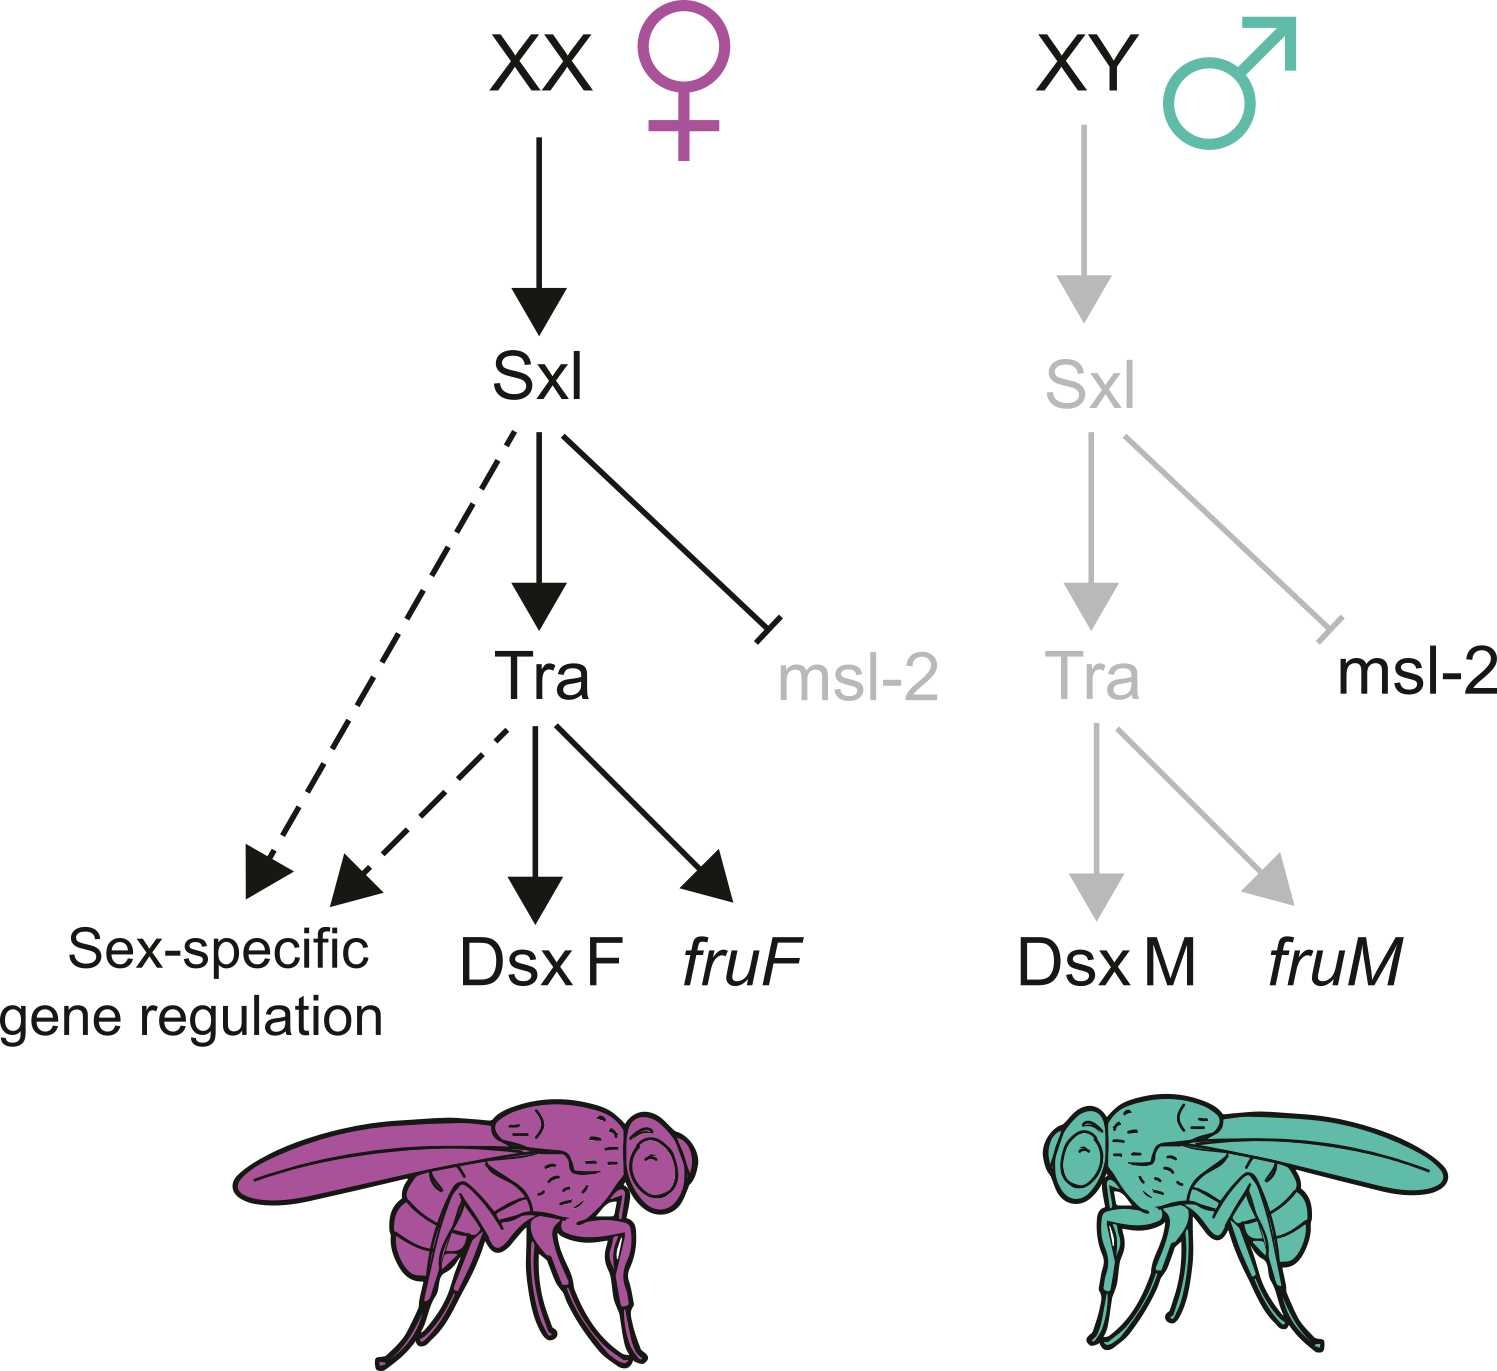
\includegraphics[width=0.5\textwidth]{sexspecifichormones.jpg}
    \caption{from Shingleton and Vea, 2023. Functional parts of the cascade are shown in black, non-functional parts are shown in gray.}
    \label{fig:label_name}
\end{figure}

\par

Sex in Drosophila is determined genetically: females possess two X
chromosomes, in addition to three autosomes, while males possess an X
and a Y chromosome. The possession of two X chromosomes leads to the
synthesis of the protein Sex-lethal (Sxl) in females only (Salz, 2011;
Shingleton \& Vea, 2023). Sxl's role in female determination is crucial
as it, directly or indirectly, initiates an expression cascade that
affects all aspects of sexual dimorphism in Drosophila (Salz, 2011). Sxl
does this by directing the synthesis of functional Transformer in
females only, through alternative splicing, which in turn directs the
alternative splicing of doublesex (dsx) and fruitless (Fru) into their
female isoforms (Salz, 2011). The female isoform of doublesex is
translated into a protein that controls the female expression of
phenotype (Deshmukh et al., 2020), while the female isoform of fruitless
is not translated into functional protein (Rideout et al., 2007). In
males, the absence of functional Tra results of the default splicing of
doublesex and fruitless into male-specific isoforms (Rideout et al.,
2007). Both are translated into protein and direct the development of
male morphology and male behavior, respectively (Rideout et al., 2007;
Shingleton \& Vea, 2023).

\par

Male and female Drosophila are therefore more-or-less genetically
identical --What is different between males and females is not so much
the genes they carry, but the genes they express. This is generally true
for all sexually dimorphic species, regardless of the genetic basis of
sex determination. Ultimately, however, these sex-specific differences
in gene expression reflect countless generations of sex-specific
selection for differences in phenotype in females and males.

\subsection{Sex-Specific Selection}

\par

Since time immemorial, the differences between females and males have
been observed. Sexual dimorphism, the morphological differences between
females and males at the same developmental stage within a species, has
been studied for well over a century. Darwin was among the first to
suggest that dimorphism evolved in response to male-male conflict and
female mating choice (1871). Since then, it has been known that sex
specific phenotypic optima also evolve in response to pressures around
courtship, mating, fecundity, parental roles, and the environment.

\par

Anisogamy, or the difference in morphology or size of female and male
gametes, is both a cause and a consequence of sex specific selection
(Fairbairn, 1997). Males produce sperm, which are small and
energetically inexpensive to produce in large quantities (Andersson,
1994; Bateman, 1948; Bjork \& Pitnick, 2006). Consequently, male
reproductive success is generally limited by his access to eggs and
females. Ova, however, are typically larger and more energetically
expensive, with females investing more to ensure offspring survival
(Andersson, 1994; Bateman, 1948). Thus, female reproductive success is
limited by fecundity, or the number of eggs females can produce.
Consequently, there is selection on males to increase their access to
females, either through male-male competition or by increasing their
`attractiveness' to females (called intrasexual and intersexual
selection respectively) (Andersson, 19994; Bateman, 1948). In contrast,
there will be selection on females to increase the number of eggs that
she can produce (called fecundity selection), and to increase the
quality of the sperm that she uses to fertilize them, and by extension
the quality of offspring these sperm help generate, by being selective
about which male(s) father her offspring (intrasexual selection)
(Andersson, 1994). The difference in gamete cost is therefore what
ultimately drives the evolution of sex specific behaviors and phenotypic
optima.

\par

Male-male intrasexual competition is common among sexual species, with
males trying to secure as many matings as possible through competition
and females mating with the most successful males. This is perhaps most
obvious in species that participate in lek mating, in which males
provide females only with gametes (Gibson \& Bradbury, 1985). Among
lekking species, members of both sexes will gather, males will compete
directly with one another through combat or elaborate displays, and
females will mate with the victorious or most attractive males
respectively.

\par

Copulation does not guarantee success, however. Among species that have
females that mate with multiple males, females may evolve mechanisms to
select which sperm she uses to fertilize her eggs. If a female's success
is predicated on having selected the best father for her offspring, her
ability to choose the father(s) of her offspring is invaluable. Hence,
in many species female choice can take place after copulating with
multiple males. For example, shortly after mating females can eject the
sperm of undesirable males. This has been observed in birds such as the
black-legged kittiwake Rissa tridactyla (Wagner et al., 2004) and the
dunnock Prunella modularis (Davies, 1983) and insects such as the flour
beetle Tribolium castaneum (Droge-Young et al., 2016) and D.
melanogaster (McDonough-Goldstein et al., 2022). Sperm can also be
subject to cryptic female choice. Cryptic female choice typically refers
to sperm selection that occurs within the female body, though it cannot
be easily observed (Birkhead, 1998). For example, in Drosophila females
select for the longest sperm (Lüpold et al., 2016). In turn, males have
evolved their own post-copulatory tools and strategies to interfere with
female choice and reduce sperm competition. To minimize sperm
competition, the males of some species will guard females during the
mating period, preventing other males from copulating (Andersson, 1994).
Mate guarding is seen in both vertebrates, particularly birds, (Sherman,
1989) and invertebrates (Simmons, 1990; Jormalainen, 1998). Another way
males can minimize sperm competition is by using mating plugs, which
block the female reproductive tract and reduce the chances of subsequent
matings resulting in fertilization. Mating plugs are common in
invertebrates including Drosophila melanogaster (Lung \& Wolfner, 2001),
but are also made by some vertebrates such as Lacerta monticola, a
species of lizard (Moreira and Birkhead, 2003). Males may also leave the
females covered in anti-aphrodisiacs, or pheromones that make females
seem unattractive, thus deterring other males from copulating with them.
Anti-aphrodisiacs are common among butterflies (Estrada et al., 2011),
but are also used by Drosophila melanogaster (Laturney \& Billeter,
2016). Some male reproductive anatomy has evolved to not only serve as a
means of insemination but also a tool to reduce sperm competition. For
example, the males of Calopteryx maculata, a species of damselfly, have
structures used during copulation to remove sperm left behind from a
female's previous matings (Waage, 1979). Intense sperm competition and
cryptic female choice can also result in evolutionary pressures on sperm
morphology and size. For example, Drosophila bifurca have sperm 5.8 cm
long, or about 20 times their body length (Lüpold et al., 2016; Pitnick
et al., 1995). Sex-specific selective pressures do not stop following
the production of offspring, as parental roles are another important
factor in reproductive success. While parental care can increase the
survival rates of offspring, each offspring adds to the burden of one or
both parents if they are not born to be self-sufficient. Females are
typically the ones shouldering this burden. Female mammals are a great
example of this, with lactation and gestation both being energetically
expensive processes. Collectively, therefore, sex-specific selective
pressures are persistent, driving evolution of increasingly complex
behavioral and morphological differences between the sexes. This
introduces potential genetic conflict in the genome for traits that are
shared by both sexes.

\subsection{Sexual Size Dimorphism}

Perhaps the most obvious form of sexual dimorphism is SSD. Female-biased
SSD (i.e., females larger than males) is common among fish, reptiles,
and arthropods, including D. melanogaster (Fairbairn, 1997; Testa et
al., 2013; Webb \& Freckleton, 2007). Male-biased SSD is common among
mammals (Fairbairn, 1997; Isaac, 2005). Rensch's rule states that among
species with female-biased SSD the degree of SSD typically decreases
with increasing species body size, while among species with male-biased
SSD the opposite is true, and SSD typically increases with increasing
species body size. A link between the evolution of sex-determination
mechanisms and that of SSD has also been suggested (Adkins-Regan \&
Reeve, 2014; Schwanz et al., 2016). Despite decades of research, there
is no consensus to explain the evolutionary mechanisms that generate
SSD. One approach to better understand these ultimate mechanisms
regulating SSD might be to focus on the proximate mechanisms regulating
SSD. While sex determination and the pressures that result in the
observed patterns of SSD have been well studied, however, how this
response occurs at a developmental genetic level remains largely
unknown.

\subsection{Developmental mechanisms regulating body size}

Generally, final body size in animals is regulated by four developmental
factors: (1) size at birth/hatching, (2) growth rate, (3) growth
duration, and (4) mass loss (Testa et al., 2013). Changes in any of
these factors alter adult body size, thus sex-specific differences in
these factors can generate SSD. Nevertheless, the molecular, genetic,
and physiological regulators of these developmental factors are poorly
understood apart from in a few model organisms. Of all animals, these
regulators are best understood in D. melanogaster which has long been
used in developmental genetics research (Shingleton \& Vea, 2023).
Drosophila is a holometabolous insect that molts through three larval
instars before pupating and metamorphosing into the final adult form.
Before pupariation, third-instar larvae must reach critical size, the
size at which larvae initiate the hormonal cascade that causes the
synthesis of ecdysone, which in turn drives metamorphosis and the
cessation of growth (Nijhout et al., 2014). The release of ecdysone
initially triggers larval wandering, which is when feeding stops and the
larvae search for a pupariation site (Nijhout et al., 2014; Testa et
al., 2013). Growth of overall body size is restricted to the larval
period, so adult body size is essentially fixed by larval body size at
pupariation (Testa et al., 2013). Thus, the factors regulating adult
body size are (1) critical size, (2) the length of time between
attaining critical size and larval wandering called the terminal growth
period (TGP), (3) the rate of growth during TGP, and (4) mass loss
during wandering (Ghosh et al., 2013; Shingleton \& Vea, 2023). Of
these, sex-specific differences in critical size, growth rate during
TGP, and mass loss appear to regulate SSD (Testa et al.,2013; Shingleton
\& Vea, 2023). We have an increasingly good understanding of the
developmental genetic mechanisms that regulate critical size, growth
rate, and mass loss. In particular, work in Drosophila over the past
three decades has illuminated the critical role the insulin/insulin-like
growth factor signaling (IIS) and Target of Rapamycin (TOR) pathways
play in regulating growth and body size. The IIS and TOR pathways are
conserved regulators of growth in metazoans, regulating growth in
response to the environment, specifically the nutritional environment
(Grewal, 2008). When nutrients are abundant, the level circulating
insulin is high and the IIS and TOR pathways promote growth. In
contrast, when nutrition is low, insulin is low and the IIS and TOR
pathways reduce their activity, suppressing growth. IIS/TOR therefore
functions not simply to regulate body size but to regulate body size in
response to the environment.

\clearpage

\textbackslash begin\{figure\}{[}h{]} \centering
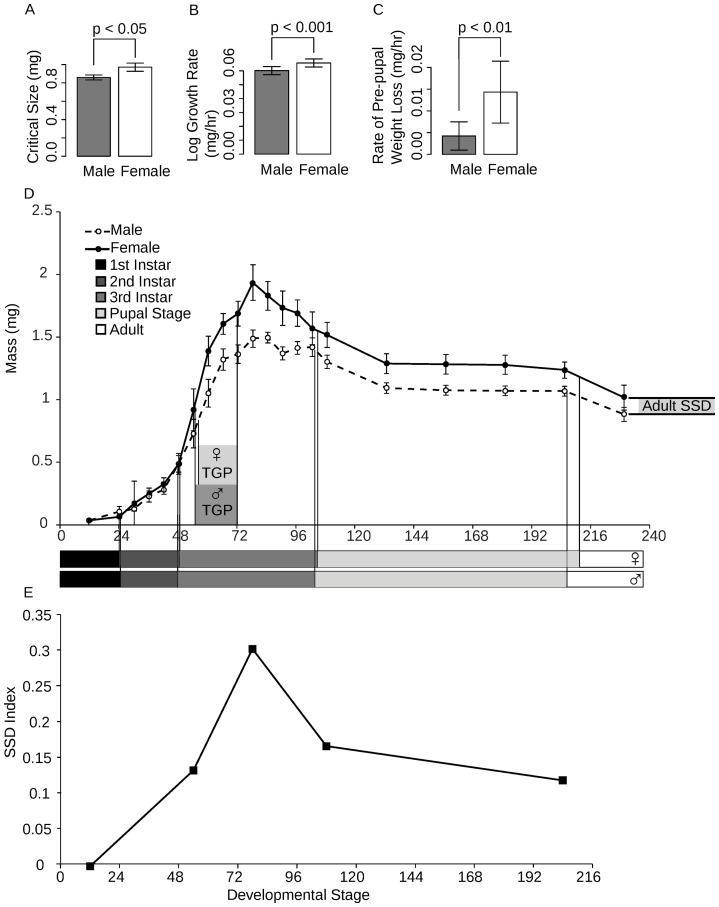
\includegraphics[width=1\textwidth]{testafig1.jpg}
\textbackslash caption\{from Testa et al., 2013. Complete growth profile
by sex for Drosophila melanogaster. Factors shown to contribute to SSD
include (a) critical size, (b) growth rate, (c) and pre-pupal weight
loss and are reflected in the sex-specific growth curve (d). The SSD at
specific developmental events (hatching, critical size, peak larval
mass, pupariation and eclosion) illustrates the changes in SSD
throughout development (e). Error bars show 95\% confidence intervals.\}
\label{fig:label_name} \textbackslash end\{figure\}

\clearpage

\subsection{Insulin is necessary for SSD}

While research over the past thirty years has increased our
understanding of the developmental-genetic mechanisms underlying body
size, how these mechanisms operate to result in SSD remains unclear. A
key discovery made by our lab, however, is that knockdown of IIS
eliminates SSD in Drosophila (Figure 2) (Testa et al., 2013). That is, a
functional IIS pathway is necessary to generate SSD. Subsequent research
suggests that females have higher levels of IIS activity than males
(Rideout et al., 2015). It follows that, since IIS activity is higher in
well-fed females than males and that knockdown of IIS eliminates SSD,
females are more sensitive to changes in IIS than males with respect to
body size. Since IIS is regulated by nutrition, it also follows that
body size in females should be more sensitive to changes in
developmental nutrition than males. That is, female body size should be
more nutritionally plastic than male body size, where plasticity refers
to the effect of the environment on phenotype independent of genotype.
This is called sex specific plasticity (SSP). Since SSP must generate
SSD, at least in some environmental conditions, observed SSD may
therefore be a consequence of selection for SSP (Shingleton \& Vea,
2023; Vea et al., 2021).

\begin{figure}[h!]
    \centering
    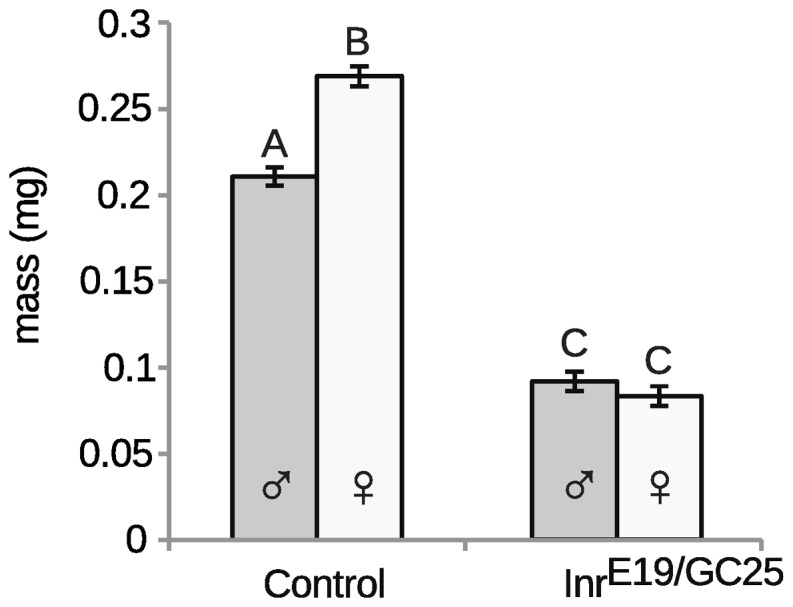
\includegraphics[width=0.5\textwidth]{testafig2.jpg}
    \caption{from Testa et al., 2013. SSD is lost in insulin-signaling mutants. The dry mass of male and female adult $Inr^{E19}$/$Inr^{GC25}$ and wild-type ($Inr^{E19}$/TM3) control flies reared at low density at 24°C. Columns with different letters are significantly different (Tukey HSD at P<0.05). Error bars are standard errors.}
    \label{fig:label_name}
\end{figure}

\subsection{Sex specific plasticity (SSP) and SSD}

The Shingleton lab has demonstrated that extensive genetic variation of
SSD is tightly correlated with sex specific plasticity (SSP) (Vea et
al., 2021). This was shown using 186 lineages from the Drosophila
Genetic Reference Panel (DGRP). The DGRP is a collection of more than
200 inbred D. melanogaster lineages generated from a wild population
from Raleigh, North Carolina after 20 generations of full sibling
inbreeding. They found that in almost all the lineages they tested,
females had higher nutritionally induced size plasticity than males (Vea
et al., 2021). Vea et al.~(2021) then went on to see how the variation
in SSP between the lineages related to the variation in SSD and found
that SSP and SSD are tightly genetically correlated. Linkage
disequilibrium breaks down over very short distances in Drosophila
(CITE), so this genetic correlation is unlikely to be due to linkage.
This suggests SSP and SSD are regulated by the same
developmental-genetic mechanisms, that is pleiotropy. Though the work of
Vea et al.~(2021) suggests overlap in the mechanisms responsible for SSP
and SSD, the loci underlying the variation they observed have yet to be
identified. Identifying the loci responsible for SSD and SSP in
Drosophila will provide insight as to how SSD and SSP (co)evolve on a
developmental-genetic level. The DGRP lineages used in by Vea et
al.~(2021) have been whole-genome sequenced, and so it is possible to
use a Genome Wide Association Study (GWAS) to identify quantitative
trait loci (QTLs) that underlie variation in SSD and SSP. This work is
ongoing.

\subsection{GWAS and E\&R are complementary approaches}

While GWAS is potentially a powerful method to identify loci that
underlie phenotypic variation it tends to favor high-frequency alleles
with large effect. A complementary approach is to investigate the
genomic response to artificial selection for change in phenotype, called
Evolve and Resequence (E\&R) (Schlötterer et al., 2015). GWAS and E\&R
have been used to identify the genes associated with Drosophila
courtship song (Turner et al., 2013). Though no single-nucleotide
polymorphisms (SNPs) were significant in either GWAS or E\&R
individually, those SNPs with high differentiation in the E\&R study
also had low P-values in the GWAS (Turner et al., 2013). As a result,
Turner et al.~(2013) were able to use both approaches to identify the
genes likely responsible for variation in courtship song. Combining GWAS
with E\&R, therefore, appears to be a potentially powerful method to
elucidate the genes that regulate SSD and SPP. Other members of the
Shingleton lab are currently using GWAS to identify genes that regulate
SSD and SSP. As a complementary approach, I will use E\&R by first
artificially selecting upon SSD (and potentially SSP) and then
identifying the loci that have been targeted (discussed further under
Aims 1 and 3).

\subsection{SSD can be changed by artificial selection}

It is not uncommon that the intensity and direction of SSD differs
between species of the same family or even genus (Fairbairn, 1997). This
suggests that SSD has considerable intraspecific variation and can be
changed by artificial selection. Tigreros \& Lewis (2011) briefly
selected on SSD of the red flour beetle Tribolium castaneum. This study
used pupal mass as the metric for body size. There were three selection
regimes, one to increase size of both sexes by selecting the largest
males and females, one to increase SSD by selecting for large females
and small males, and one to reduce SSD by selecting for small females
and large males. However, they were not successful after applying
selection for only seven generations as both sexes experienced a similar
increase or decrease in mass with each generation in all lines. Stewart
\& Rice (2018) selected on D. melanogaster size over 250 generations.
They used a sieve-sorter to quickly separate adults each generation by
body size. There were four treatments: Controls (no selection); sex
concordant-large (selection for large body size in both sexes); sex
concordant-small (selection for small body size in both sexes); and sex
discordant (selection for large males and small females). After about
175 generations of sex discordant selection, they were able to reverse
the direction of SSD from female-biased to male-biased (that is from
females being the larger sex, to males being the larger sex). As
incredible as those results are, to conduct a selection experiment that
large over that many generations, it is not feasible for a PhD student
to undertake. Bird and Schaffer (1972) successfully artificially
selected on the magnitude of sexual dimorphism of the wings of D.
melanogaster nearly fifty years ago. Because sexual dimorphism is a
group trait, their selection regime utilized family selection. After
only fifteen generations, they generated two lineages, one of increased
wing sexual dimorphism and one of reduced sexual wing dimorphism. After
ten generations of relaxed selection, the lineages maintained increased
and reduced wing dimorphism respectively. Thus, Bird and Schaffer must
have successfully targeted the developmental-genetic mechanisms
responsible for the sex specific difference in wing size. Bird and
Schaffer's research was conducted at a time when our understanding of
developmental mechanisms and genetics was limited, and it was impossible
to identify the mechanisms responsible for the difference they observed.
Because of Bird and Schaffer's (1972) straightforward selection regime
and rapid response, however, their work inspired much of how I
approached Aim 1. While these artificial selection studies attempted to
modify dimorphism, and some attempted to modify SSD specifically, the
means of measuring (torso size or width) do not reflect overall body
size as effectively as pupal area. These studies also did not trace
pedigree, whereas my work can trace all ancestors, providing some
insight into degree of inbreeding and potentially which individuals
contributed the most to changes in final SSD.

\bibliography{export.bib}

\end{document}
